\chapter{Implementáció}
\textbf{Megjegyzés: a leírt lépések során feltételezem, hogy a számítógépen telepítve van \textit{docker} (kliens és motor egyaránt), illetve \textit{kubectl}\footnote{Kubernetes menedzsment eszköz} és \textit{awscli}\footnote{AWS parancssori alkalmazás}.}
\vskip 0.1in
Az előzetes tervezésem eredményeképp megállapítottam hogy mire lesz szükségem. Tudtam, hogy a Kubernetes lesz a fő "összetevő" hiszen a skálázás és a szolgáltatás alapvető monitorozása könnyen megvalósítható benne. CI/CD vonatkozásában több lehetőségem is volt, de a konzulensemmel történt egyeztetés alapján a Jenkinsre esett a választás. Noha külön virtuális gépre is helyezhettem volna, én a praktikusság kedvéért mindent egy klaszterre szerettem volna telepíteni, és ez így is történt. További alapvető teendőim voltak (bár ez a feladatkiírásban nem szerepelt) a klaszterszintű monitorozás megvalósítása. Ezt Prometheus és Grafana segítségével szerettem volna megvalósítani, melybe később a szolgáltatások is beköthetőek lehetnek.
\section{Alkalmazás Docker konténerekbe helyezése}
A Kubernetes Dockerre épül és az alkalmazások "telepítése" is konténerképek formájában történik, így hát legelső lépésben az alkalmazáskomponenseket kellett konténerizálnom, szerencsére az már funkcionalitás szerint frontendre és backendre volt bontva.

Azt hamar eldöntöttem, hogy a programkód fordítását és futtatását is Dockerben szeretném végezni, így éltem az úgynevezett \textit{Multi-stage build}\cite{multistage_docker} adta lehetőséggel miszerint több konténert is felhasználhatunk egy adott konténerkép előállításához. Ekkor ez utolsó konténerkép "rész" lesz az amit a konténer indításakor végrehajtunk. Esetemben kell egy konténer amiben a fordítás (\textit{build}) zajlik és egy másik ami a futtatókörnyezet. A fordítás az egyszerűbb művelet, legalábbis konténerizáció szempontjából. Az én esetemben a frontendet \textit{npm} programmal kellett fordítani, melyre kész konténer áll rendelkezésre \textit{node} néven. Ebbe a konténerbe kell másolni a forráskódot, majd a megfelelő parancsot kiadni. A backend esetén hasonló a lépés, ott a \textit{maven} konténerből érdemes kiindulni.

Előálltak a futtatandó alkalmazáskomponensek, azonban azoknak is meg kell határozni a futtatókörnyezetet: a frontend esetén erre a \textit{serve} csomagot alkalmaztam ami az npm csomagkezelővel letölthető, így itt is a \textit{node} konténerképből indultam ki. A backend esetében a fordítás produktuma egy darab \lstinline{.jar} fájl amihez Java 11 futtatókörnyezet volt szükséges: az \lstinline{openjdk:11} konténerképet választottam. Ezekbe át kell másolni a futtatáshoz szükséges fájlokat, aztán már csupán a hálózati kommunikációt szükséges megoldani. Ezt a Dockerfile \lstinline{EXPOSE} parancsa félig megoldja, paraméterül a portszámot várja amin alkalmazásunk figyel. Ne felejtsünk el a végén \lstinline{ENTRYPOINT}-ot megadni, tehát azt a parancsot amit a konténer indulásakor az végrehajt.

Íme a backend Dockerfileja (\textit{a többi is megtalálható a dolgozat GitHub repositoryjában}):
\begin{lstlisting}
FROM maven:latest as build # a fordítókörnyezet konténerképe
WORKDIR /usr/src/mymaven
COPY pom.xml ./            # a programkód másolása
COPY src/ src/
RUN ["mvn", "package"]     # a fordításra szolgáló parancs megadása

FROM openjdk:11 as runner  # a futtatókörnyezet konténerképe
WORKDIR /usr/src/webshop   
COPY --from=build /usr/src/mymaven/target/*.jar ./webshop.jar # lefordított kód másolása
EXPOSE 8081                # a port használatának jelzése
ENTRYPOINT ["java","-Djava.security.egd=file:/dev/./urandom","-jar","webshop.jar"]
\end{lstlisting}

Az alkalmazás természetesen lokálisan is tesztelhető. Csinálni kell egy hálózatot, amihez a konténereket csatoljuk. A konténerek neve legyen rendre: frontend, backend, database. (Természetesen ez csak a példaalkalmazás esetében igaz, de az elv ugyanaz: Kubernetesbe helyezés elett célszerű Dockerben összeépíteni az egész alkalmazást és kipróbálálni azt.)
\section{Felhő-infrastruktúra kialakítása}
A feladatkiírás szerint az Amazon Web Services adta Kubernetes szolgáltatást (EKS) kellett használnom. Praktikus okokból mindent az AWS rendszerében építettem ki, mely korántsem olyan egyszerűen átlátható elsőre, mint például a Google Cloud Platform.
\subsection{Kubernetes klaszter építése}
Mielőtt a klaszter létrehozását elkezdenénk szükséges létrehoznunk egy új IAM szerepet. Ezt az AWS konzol IAM felületén tehetjük meg a \textbf{Roles} nézetben a \textbf{Create Role}ra kattintva. Válasszük ki, hogy Amazon szolgáltatásnak szánjuk a szerepet majd válasszük ki az \textbf{EKS}t. Kettő szabály kerül hozzáadásra, ezt majd még később bővítjük, egyenlőre elég ennyi. A következő oldalon címkéket rendelhetünk a szerephez. Bár itt most nagy jelentősége nincs, azonban például egy virtuális gépet (EC2 példány) célszerű megcímkézni ugyanis így a költségek konzolján hatékonyan lehet keresni például hogy egy adott szolgáltatásunk mennyibe kerül. Adjunk egy tetszőleges nevet a következő nézetben.

A klaszter létrehozásához szükségünk van még egy VPCre is, azonban az Amazon alapértelmezetten konfigurál egyet ami a mi felhasználásunkra most tökéletes is lesz. Hozzuk létre a klasztert:
\begin{enumerate}
    \item Lépjünk az EKS konzolra és kattintsunk a \textbf{Create cluster} gombra.
    \item Adjunk egy nevet a klaszternek, válasszuk ki a kívánt verziót (én a pillanatyni legfrissebb elérhető verziót, az 1.14-t választottam), illetve a fentebb készített szerepet rendeljük a klaszterhez.
    \item A hálózatok fülön válsszuk ki az alapértelmezett VPC-t, biztonsági csoportot, illetve engedélyezzük a publikus API szerver hozzáférést, hogy a saját számítógépünkről menedzselni tudjuk a klasztert.
    \item A logolásnál alapértelmezetten én kikapcsolva hagytam mindent, költséghatékonysági okokból (a logolás és annak tárolása is költségelem). Nem lesz rá szükségünk, azonban - ahogyan én is tettem - a hibakeresést meg tudja könnyíteni például az API server logolás bekapcsolása.
    \item Adjunk címkét a klaszternek, itt már erősen ajánlott, hiszen havi 144 amerikai dollárt tesz majd hozzá a havi számlához.
    \item Kattintsunk a \textbf{Create} gombra.
\end{enumerate}

A klaszterünk elkészült, azonban még nem tudjuk menedzselni a gépünkről. Ehhez szükséges a \textit{kubectl} és az AWS hozzáférés konfigurálása. Utóbbihoz az \textit{awscli} eszköz beszerzése szükséges melynek legegyszerűbb módja futtatni a \lstinline{pip3 install awscli --user --upgrade} parancsot. Használat előtt csinálnunk kell egy hozzáférési kulcsot AWS fiókunkhoz. Ezt a webes konzolon tehetjük meg a fióknevünkre kattintva és ott a \textbf{My Security Credentials} pontot választva. Itt csináljunk egy kulcsot a \textbf{Create access key} gombra kattintva, és \textit{ne} zárjuk be az ablakot. Egy terminálablakba írjuk be, hogy \lstinline{aws configure}, majd rendre adjuk meg a hozzáférési kulcs azonosítóját, magát a kulcsot, az alapértelmezett régiót, illetve a kimenet alapértelmezett formátumát, mely praktikusan nálam \lstinline{text} értékre lett állítva. Ezzel parancssori hozzáférést szereztük fiókunkhoz, és nincs más hátra mint a kubectl eszközt konfigurálni. Ehhez szerencsére az AWS programja segítséget nyújt egy beépített paranccsal: \lstinline{aws eks update-kubeconfig --name a_klaszter_neve}. Készen is vagyunk, hozzáférünk a Kubernetes klaszterhez, azonban még nincsen \textit{worker} csatlakoztatva, így nincs hol futtatni az alkalmazásokat.
\subsubsection{Workerek létrehozása}
Ahhoz hogy egy használható Kubernetes klaszterünk legyen, szükség van olyan kiszolgálókra melyeknek a szolgáltatások futtatása a feladatuk. Ezeket \textit{worker}eknek hívják, és az AWS webes felületén pár kattintással létrehozhatjuk azokat. Az EKS konzolon válasszuk a \textbf{Create node group} opciót majd a megjelenő ablakban adjunk nevet a workerek csoportjának, válasszük ki a hozzájuk rendelendő szerepet (alapértelmezetten létezik egy \textit{NodeInstanceRole} ez teljesen megfelel a célnak) és jegyezzük meg, ugyanis később még ezt konfigurálni kell. A \textbf{Subnets} résznél válasszük ki mindhármat (ez az alapértelmezett VPC három elérhetőségi zónában lévő egy-egy alhálózata). A kiszolgálókhoz nincs szükségünk távoli elérésre, vegyük ki a jelölőnégyzetből a pipát (Itt lenne lehetőség SSH\footnote{Secure Shell - távoli parancssoros elérés} elérést konfigurálni, azonban mi kizárólag kubectl segítségével fogjuk menedzselni ezeket a gépeket. Haladó szintű hibakereséshez vagy helyreállításhoz azonban hasznos lehet engedélyezni.). A \textbf{Tags} résznél érdemes címkézni őket, a fentebb említett okok miatt. Kattintsunk a \textbf{Next} gombra és állítsuk be a használni kívánt EC2 géptípust. Válasszunk egy AMI-t\footnote{Amazon Machine Image - meghatározza az operációs rendszert, előtelepített programokat és konfigurációt}, érdemes az új, \textit{Amazon Linux 2}-t választani. A példány típusát az igények szerint érdemes választani, azonban vegyük figyelembe, hogy érdemes legalább három workert futtatni egyidejűleg, illetve azt is, hogy nem érdemes 4-8GB-nál kevesebb memóriával rendelkező típust választani. Szakdolgozatom készítése során én a \textit{t3.medium}-ot választottam, és 20GB lemezterületet allokáltam minden kiszolgálónak.

A következő fülön az automatikus skálázást lehet konfigurálni:
\begin{itemize}
    \item Minimum size - A klaszterben minimálisan létező kiszolgálók száma, érdemes legalább három gépet fenntartani. Én a dolgozat írása során kettőre állítottam. A döntésemet lentebb indoklom.
    \item Maximum size - A klaszterben maximálisan létező kiszolgálók száma. Ezt a számot kizárólag az igények (és a pénztárca) határozza meg, én négyet határoztam meg.
    \item Desired size - A kívánt méret, gyakorlatilag csak a létrehozáskor van jelentősége, aztán az Amazon kiszámolja, hogy a min-max között mi lenne az optimális, és beállítja.
\end{itemize}
Természetesen az automatikus skálázás kikapcsolható ha mindhárom értéket ugyanarra konfiguráljuk.

Egy kis kitérőt teszek hogy megértsük miért csupán két gépet használok annak ellenére, hogy többször is írtam, hogy hármat ajánlott. Ennek leginkább költséghatékonysági okai vannak, ugyanis felesleges ténylegesen három példány, egy viszont nagyon szűkös lenne. Kettő ideális abból a szempontból, hogy olcsóbb mint három, viszont lehet tesztelni a migrációt és az erőforráshasználat optimalizálását. Éles, klaszterezett rendszerekben ajánlott páratlan számú kiszolgálót futtatni, két gépet pedig egyenesen nem ajánlott. Ez a \textit{Split Brain} probléma elkerülése végett van így. Split Brainnek nevezik azt amikor létezik mondjuk két kiszolgáló és megszakad a kettő között a kommunikáció. Ekkor mindkét fél azt hiszi, hogy a másik üzemképtelen, ezért a magas rendelkezésreállás biztosítása miatt elkezdik ugyanazt a feladatot ellátni, ezzel inkonzisztenciát okozva.

A skálázás konfigurálása után már csak át kell néznünk a beállításainkat és a \textbf{Create} gombra kattintva érvényesíteni azokat. Kis idő elteltével elérhetőek lesznek a kiszolgálók. Ezt a \lstinline{kubectl get nodes} paranccsal ellenőrizni is tudjuk.
\subsection{Konténerkép-tároló kialakítása}
Az korábban említettem, hogy a Kubernetes Docker konténereket futtat és ehhez egy konténerkép-tárolóra is szükség van. Természetesen használhatnánk a nyílt és ingyenes Docker Hubot, azonban ezt azt jelentené hogy azok mindenki számára elérhetőek lesznek. Vállalati felhasználásra praktikusabb egy privát tárolót használni, ráadásul az Amazon saját tárolójával az általuk nyújott Kubernetes szolgáltatás jól integrálódik.

Az \textit{Elastic Container Registry (ECR)} használatához két dologot kell tennünk: létrehozni a konténerképenkénti repositorykat illetve hozzáférést garantálni a dologozó kiszolgálók számára.

A repositoryk létrehozása nagyon egyszerű dolog, látogassuk meg az ECR webkonzolt, majd kattintsunk a \textbf{Create repositry} gombra. Itt adjunk egy nevet (én praktikusan az alkalmazás\_neve-komponens\_neve sémát követtem (pl.: webshop-backend)), illetve határozzunk meg két opciót:
\begin{itemize}
    \item Tag immutability - Azt határozza meg, hogy a tagek felülírhatóak legyenek-e. Ennek például akkor van jelentősége ha szeretnénk \lstinline{:latest} taget használni ami mindig felülíródik a legutolsó build alkalmával. Én kikapcsoltam ugyanis kizárólag build ID-kat használok amiknek nem szabad megegyezniük mivel minden fordítás alkalmával növekedő számról beszélünk.
    \item Scan on push - Azt határozza meg, hogy amikor egy új konténerképet töltünk fel, akkor az Amazon átnézze-e a repositoryt. Ennek a webfelületen van jelentősége, ugyanis például a szolgáltatás sérülékenység-analalízist is biztosít. Explicit kérésnél (például egy docker pull kép:tag esetén) nincs jelentősége. Én kényelmi okokból bekapcsoltam, plusz költséggel nem jár.
\end{itemize}

Az utolsó lépés a hozzáférés engedélyezése az EKS számára (hogy ténylegesen tudják használni a privát kontérnerképeinket). Ehhez az IAM konzolon kell létrehoznunk egy új \textit{Policy}t. Adjunk neki egy nevet, például \lstinline{ECR_read}, és állítsuk be a következő JSON értéket\cite{ECR_IAM}:
\newpage
\begin{lstlisting}
{
    "Version": "2012-10-17",
    "Statement": [
        {
            "Effect": "Allow",
            "Action": [
                "ecr:BatchCheckLayerAvailability",
                "ecr:BatchGetImage",
                "ecr:GetDownloadUrlForLayer",
                "ecr:GetAuthorizationToken"
            ],
            "Resource": "*"
        }
    ]
}
\end{lstlisting}
Ez olvasási hozzáférést garantál minden ECR-ben lévő konténerképhez. Keressük meg a NodeInstanceRole szerepet, és rendeljük hozzá ezt az új szabályt (\textbf{Attach Policy}). Egy-két perc elteltével már hozzá is férhetünk a konténerképekhez.
\subsection{Pod szintű hozzáférés-szabályozás kialakítása}
Később a Jenkins számára írási jogokat is kell adni, így praktikusan készítsünk egy szerepet erre a célra. Csináljunk egy új policyt az alábbi JSON adatokkal, nevezzük mondjuk \lstinline{EKS_write}nak:
\begin{lstlisting}
{
    "Version": "2012-10-17",
    "Statement": [
        {
            "Effect": "Allow",
            "Action": [
                "ecr:GetAuthorizationToken",
                "ecr:BatchCheckLayerAvailability",
                "ecr:GetDownloadUrlForLayer",
                "ecr:GetRepositoryPolicy",
                "ecr:DescribeRepositories",
                "ecr:ListImages",
                "ecr:DescribeImages",
                "ecr:BatchGetImage",
                "ecr:GetLifecyclePolicy",
                "ecr:GetLifecyclePolicyPreview",
                "ecr:ListTagsForResource",
                "ecr:DescribeImageScanFindings",
                "ecr:InitiateLayerUpload",
                "ecr:UploadLayerPart",
                "ecr:CompleteLayerUpload",
                "ecr:PutImage"
            ],
            "Resource": "*"
        }
    ]
}
\end{lstlisting}
Ez olvasási és írási jogokat is garantál, azonban repositoryk törlésére még alkalmatlan.

Ahhoz hogy a pod authentikálni tudja magát, létre kell hoznunk egy OpenID szolgáltatót. Erre a legegyszerűbben egy konzolos eszközzel van lehetőségünk, az \lstinline{eksctl} nevű eszközzel. Ennek telepítése:
\begin{lstlisting}
curl --silent --location "https://github.com/weaveworks/eksctl/releases/download/latest_release/eksctl_$(uname -s)_amd64.tar.gz" | tar xz -C /tmp
sudo mv /tmp/eksctl /usr/local/bin
\end{lstlisting}

Most már létrehozhatunk egy szolgáltatót\cite{OIDC_IAM}:
\begin{lstlisting}
eksctl utils associate-iam-oidc-provider \
               --name a_klaszter_neve \
               --approve
\end{lstlisting}
Csináljunk egy új szerepet mondjuk JenkinsRole néven. Az entitás típusának válasszuk a \textbf{Web identity} típust. A szolgáltató legyen az \textbf{oidc} kezdetű, a közönség pedig \textbf{sts.amazonaws.com} majd a következő oldalon csatoljuk hozzá a fentebb készített szabályt. Ezzel a szerep elkészült, a Jenkins telepítésénél egyszerű dolgunk lesz.
\section{Ingress Controller telepítése}
Ahhoz hogy a klaszterünket a külvilág felől el lehessen érni (menedzsment felhasználáson kívül) Ingressek definiálására van szükség. Ezek viszont csak akkor működnek ha egy úgynevezett Ingress Controller is telepítve van. A Kubernetes jelenleg két fajta vezérlőt támogat\cite{ingresscontroller_k8s} melyek közül én az Nginx Ingress Controllert válaszottam.
\begin{figure}[ht]
\centering
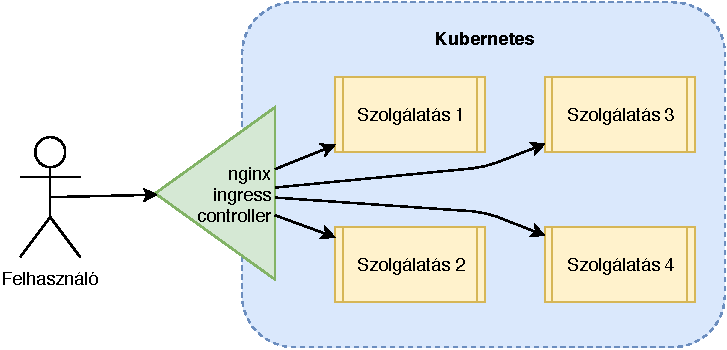
\includegraphics[width=110mm, keepaspectratio]{img/nginx_controller.pdf}
\caption{A Ingress Controller működése}
\end{figure}
\vskip 0.1in
A telepítés összesen két parancsot igényel mivel egyedi konfigurációt csak az Ingressek fognak tartalmazni. Az alábbi utasításokat adjuk ki:
\begin{lstlisting}
kubectl apply -f https://raw.githubusercontent.com/kubernetes/ingress-nginx/master/deploy/static/mandatory.yaml
kubectl apply -f https://raw.githubusercontent.com/kubernetes/ingress-nginx/master/deploy/static/provider/aws/service-nlb.yaml
\end{lstlisting}
Ezzel el is készült egy Elastic Network Load Balancer (NLB). Minden ide érkező kérést a megfelelő Podnak továbbít a vezérlő. De mi is az az "ide"? Az alábbi paranccsal nézzük meg:
\begin{lstlisting}
kubectl get services -n ingress-nginx

nginx-ingress-controller   LoadBalancer   10.100.253.39   ac...21.elb.eu-central-1.amazonaws.com 
80:32645/TCP,443:30928/TCP
\end{lstlisting}
A lényeg a \textbf{xxx.elb.yyy.amazonaws.com} cím. Erre célszerű úgynevezett CNAME-t felvenni a DNS\footnote{Domain Name System - domainok nevét fordítja IP címre} rekordok közé. A CNAME gyakorlatilag egy domaincímről egy másikra hivatkozó bejegyzés, melyet könnyű felismerni. Esetemben például így néz ki:
\begin{lstlisting}
host webshop.mbraptor.tech

webshop.mbraptor.tech is an alias for szakdolgozat.mbraptor.tech.
szakdolgozat.mbraptor.tech is an alias for ac...21.elb.eu-central-1.amazonaws.com.
ac...21.elb.eu-central-1.amazonaws.com has address 3.125.68.208
\end{lstlisting}
Azért van szükség erre, és nem közvetlenül az IP címre hivatkozni, mert az egy változó cím. Ezért ad az Amazon egy fix bejegyzést amit karban tart. Az \lstinline{mbraptor.tech} a saját domainem, melynek konfigurációját én kezelem.
Tehát elértük, hogy a szolgáltatásaink elérhetőek legyenek az internet felől. Azonban a klaszterünkben még semmi nem fut, csupán egy "404 Nem található" hibaüzenetet kapunk.
\section{Monitorozás kialakítása}
Monitorozás alatt most magának a klaszternek a monitorozását értem (bár a szolgáltatások erőforráshasználatára ez például tökéletesen alkalmas). Ezt végtelenül egyszerű lesz telepíteni a \textit{Helm} segítségével, ami lényegében egy Kubernetes csomagkezelő. Ezt viszont telepíteni kell a számítógépünkre:
\begin{lstlisting}
curl https://raw.githubusercontent.com/helm/helm/master/scripts/get-helm-3 > get_helm.sh
chmod 700 get_helm.sh
./get_helm.sh
\end{lstlisting}
A parancs futtatása után zárjuk be a terminálablakot és nyissuk meg újra. A Helm használatra kész.

Innen a fentebb ismertetett Prometheus monitorozó rendszer telepítése szó szerint két sor:
\begin{enumerate}
    \item Csináljunk egy namespacet a monitorozással kapcsolatos szolgáltatásoknak: \lstinline{kubectl create namespace monitoring}
    \item Telepítsük a Prometheust: \lstinline{helm install --name prometheus stable/prometheus --namespace monitoring}
\end{enumerate}

Most már a klaszterről tárolódnak a metrikák, azonban még megtekinteni nem lehet azt (legalábbis felhasználóbarát felületen nem). Ehhez a Grafana webalkalmazásra lesz szükség, melynek telepítése szintén egyszerű, de többletkonfigurációt igényel. Egyrészt be kell állítani adatforrásnak a Prometheust, illetve konfigurálni kell a Grafana perzisztenciát (hogy az esetleges módosítások ne tűnjenek el ha a Pod áthelyeződik). Ehhez két fájlt kell létrehozni az alábbi tartalommal:

grafana.yaml
\begin{lstlisting}
apiVersion: v1
kind: ConfigMap
metadata:
  name: prometheus-grafana-datasource
  namespace: monitoring
  labels:
    grafana_datasource: '1'
data:
  datasource.yaml: |-
    apiVersion: 1
    datasources:
    - name: Prometheus
      type: prometheus
      access: proxy
      orgId: 1
      url: http://prometheus-server.monitoring.svc.cluster.local
\end{lstlisting}
grafana-values.yaml
\begin{lstlisting}
sidecar:
  datasources:
    enabled: true
    label: grafana_datasource

persistence:
  enabled: true
  storageClass:
  annotations: {}
  accessMode: "ReadWriteOnce"
  size: "8Gi"
\end{lstlisting}
Illetve definiálnunk kell egy Ingress-t is, hogy melyik cím legyen a Grafanára irányítva. Én konfiguráltam a HTTPS kapcsolatot is, ez ugyan nem szükséges, de éles rendszerben ajánlott. Természetesen a tanúsítványt nem teszem közzé, azt fájlból is hozzá lehet adni, vagy base64 enkódolással a konfigurációba írni helyezni azt.

ingress.yaml
\begin{lstlisting}
apiVersion: networking.k8s.io/v1beta1
kind: Ingress
metadata:
  name: monitoring
  annotations:
    kubernetes.io/ingress.class: "nginx"
    nginx.ingress.kubernetes.io/force-ssl-redirect: "true"
spec:
  tls:
  - hosts:
    - szakdolgozat-monitoring.mbraptor.tech
    secretName: tls-mbraptor.tech
  rules:
  - host: szakdolgozat-monitoring.mbraptor.tech
    http:
      paths:
      - backend:
          serviceName: grafana
          servicePort: 80

---

apiVersion: v1
kind: Secret
data:
  tls.crt: ...
  tls.key: ...
metadata:
  name: tls-mbraptor.tech
type: kubernetes.io/tls
\end{lstlisting}
Ezeket a fájlokat már csak alkalmazni kell a \lstinline{kubectl apply -n monitoring -f FILENAME.yaml} paranccsal. Ha mindent jól csináltunk akkor a beállított oldalon (esetemben \url{szakdolgozat-monitoring.mbraptor.tech}) már elérhető a Grafana, a Helm telepítés végén található adminisztrátori adatokkal beléphetünk. A Grafana beállítása szakdolgozatomnak nem témája, de a \textit{Dashboard import} funkcióval és az \url{https://grafana.com/grafana/dashboards} oldalon található kész elrendezések jó kiindulási alapot jelenthetnek.
\section{Jenkins telepítése}
A Jenkins telepítését szintén Helm segítségével fogjuk végezni, azonban itt nagyobb mértékű konfigurációra lesz szükség. Egyrészt mivel a Jenkins közvetlenül fogja a Kubernetes API-t hívni ezért jogosultságokat kell adni neki, továbbá az alapértelmezett Jenkins konténerkép helyett is sajátot használok, illetve a fentebb beállított IAM szerepet is fel kell konfigurálni az AWS API kommunikációhoz.

Kezdetnek adjunk jogosultságot a Jenkinsnek. Ennek hozzunk létre egy fájlt péládul \lstinline{eks-jenkins-rbac.yaml} néven:
\begin{lstlisting}
kind: ClusterRole
apiVersion: rbac.authorization.k8s.io/v1
metadata:
  name: jenkins-role-cluster
rules:
- apiGroups:
  - ""
  - "apps"
  - "networking.k8s.io"
  - "autoscaling"
  resources:
  - pods
  - configmaps
  - deployments
  - secrets
  - services
  - ingresses
  - apps
  - horizontalpodautoscalers
  - statefulsets
  verbs:
  - create
  - delete
  - deletecollection
  - get
  - list
  - patch
  - update
  - watch

---

apiVersion: rbac.authorization.k8s.io/v1
kind: RoleBinding
metadata:
  name: jenkins-role-prod
  namespace: webshop-prod
roleRef:
  apiGroup: rbac.authorization.k8s.io
  kind: ClusterRole
  name: jenkins-role-cluster
subjects:
- kind: ServiceAccount
  name: ci-jenkins
  namespace: szakdolgozat-aws

---

apiVersion: rbac.authorization.k8s.io/v1
kind: RoleBinding
metadata:
  name: jenkins-role-beta
  namespace: webshop-beta
roleRef:
  apiGroup: rbac.authorization.k8s.io
  kind: ClusterRole
  name: jenkins-role-cluster
subjects:
- kind: ServiceAccount
  name: ci-jenkins
  namespace: szakdolgozat-aws
  ...
\end{lstlisting}
Mivel a Jenkins több névtérben is dolgozik, így egy klaszterszintű jogosultságot definiálunk (\textit{ClusterRole}), és ezt érvényesítjük adott névterekre (\textit{RoleBinding}), jelen esetben az alkalmazás két névterére.
Hozzuk létre a szóban forgó namespaceket és alkalmazzuk a konfigurációt:
\begin{lstlisting}
kubectl create namespace szakdolgozat-aws #ennek az elnevezésnek történelmi okai vannak, természetesen lehet jenkins is a neve
kubectl create namespace webshop-beta
kubectl create namespace webshop-prod

kubectl apply -n szakdolgozat-aws -f eks-jenkins-rbac.yaml
\end{lstlisting}
Ezzel a Kubernetes felé történő kommunikáció engedélyezve van, és a Jenkins által használt műveletek engedélyezve vannak (de természetesen ez alkalmazásfüggő). Szükséges még egy Ingress is: teljesen ugyanazt a műveletet kell elvégezni, amit a Grafana esetében (értelemszerűen a cím átírandó). Mivel konfigurált Jenkinst szeretnénk így a Helm telepítés előtt el kell készítenünk azt. Töltsük le az alábbi fájlt: \url{https://github.com/helm/charts/tree/master/stable/jenkins} és mentsük el \lstinline{jenkins-values.yaml} néven. Írjunk át benne pár dolgot:
Módosítsuk az alábbiakat, hogy az általam készített \textit{kubectl} és \textit{docker} klienssel ellátott konténerképet használja a telepítés.
\begin{lstlisting}
...
master:
  # Used for label app.kubernetes.io/component
  componentName: "jenkins-master"
  image: "msbence/jenkins-docker-kubectl"
  tag: "aws"
...
\end{lstlisting}
Adjuk hozzá környezeti változóként, hogy TCP kapcsolaton keresztül érjük el a Docker motort, továbbá adjuk meg azt az URL-t ahol a Jenkins elérhető lesz.
\begin{lstlisting}
...
initContainerEnv:
    - name: DOCKER_HOST
      value: "tcp://localhost:2375"
  containerEnv:
    - name: DOCKER_HOST
      value: "tcp://localhost:2375"
  # Set min/max heap here if needed with:
  # javaOpts: "-Xms512m -Xmx512m"
  # jenkinsOpts: ""
  jenkinsUrl: "https://ci.mbraptor.tech"
  # If you set this prefix and use ingress controller then you might want to set the ingress path below
...
\end{lstlisting}
Pár plugint telepítenünk kell az alapértelmezetteken túl. A \textit{BlueOcean} a Jenkins egy új, kísérleti felülete mely nagyban megkönnyíti annak használatát. A \textit{locale} plugin segítségével beállíthatunk nyelvet a szoftvernek ugyanis alapértelmezetten a böngésző által küldöttet használja, azonban a Jenkins magyar fordítása nem megfelelő minőségű. Az \textit{Amazon ECR} pedig a konténerképek feltöltésénél segít.
\begin{lstlisting}
...
  # List of plugins to be install during Jenkins master start
  installPlugins:
    - kubernetes:1.21.3
    - workflow-job:2.36
    - workflow-aggregator:2.6
    - credentials-binding:1.20
    - git:4.0.0
    - blueocean:1.19.0
    - locale:1.4
    - amazon-ecr:1.6
...
\end{lstlisting}
Fentebb hivatkoztunk egy Docker motorra melyet ez a konténer valósít meg. Ez egy \textit{Docker-in-Docker} konténerkép a hivatalos Docker csapat által támogatva.
\begin{lstlisting}
...
sidecars:
    configAutoReload:
    ...
    other:
     - name: docker-daemon
       image: docker:18.09-dind
       resources:
        requests:
          cpu: 50m
          memory: 512Mi
        limits:
          cpu: 2000m
          memory: 2048Mi
       securityContext:
           privileged: true
       volumeMounts:
                 - name: docker-graph-storage
                   mountPath: /var/lib/docker
...
\end{lstlisting}
Ahhoz hogy ne lássuk a gazdagép (Kubernetes worker node) Docker adatait egy üres tárolót kell csatolnunk, ezzel elfedve azokat.\cite{dind_ci}
\begin{lstlisting}
...
persistence:
  enabled: true
  existingClaim:
  storageClass:
  annotations: {}
  accessMode: "ReadWriteOnce"
  size: "8Gi"
  volumes:
      - name: docker-graph-storage
        emptyDir: {}
networkPolicy:
...
\end{lstlisting}
Ahhoz hogy a Pod hozzáférjen az AWS APIhoz a megfelelő szerepet kell kapnia. A fentebb létrehozott JenkinsRole szerepet állítsuk be az alábbi módon:
\begin{lstlisting}
...
rbac:
  create: true
  readSecrets: false

serviceAccount:
  create: true
  # The name of the service account is autogenerated by default
  name:
  annotations:
    eks.amazonaws.com/role-arn: "arn:aws:iam::123456789:role/JenkinsRole"

serviceAccountAgent:
...
\end{lstlisting}
A konfigurálást befejeztük, most már tényleg csak a Helm telepítést kell lefuttatni és szinte kulcsrakész Jenkinst kapunk fáradozásainkért cserébe. A parancs a Grafanához hasonló: \lstinline{helm install --name ci --namespace szakdolgozat-aws stable/jenkins -f jenkins-values.yaml}

Kis idő elteltével a Jenkins elérhető az Ingressnél megadott címen, az adminisztrátori jelszó megszerzéséről pedig a Helm tájékoztat. Belépés után a Jenkins kezelése (\textbf{Manage Jenkins}) menüben keressük meg a \textbf{Locale} plugin részét a \textbf{Rendszer kezelése} pont alatt és állítsuk a nyelvet \lstinline{en_US}-ra, valamit jelöljük be a \textbf{Ignore browser preference and force this language to all users} jelölőnégyzetet. Kattintsunk az \textbf{Apply} gombra és most már angol nyelvű felület fogad minket.

További hasznos teendő ha a \textbf{Manage Jenkins} menü alatt a \textbf{Global Security} menüben a \textbf{Security Realm}ot átállítjuk a Jenkins saját adatbázisára, ekkor lesz lehetőségünk több felhasználót hozzáadni, jelszót cserélni, stb...

Annak érdekében, hogy a Jenkins Docker támogatását könnyen használni tudjuk még be kell állítanunk az ECR hozzáférést is. Ezt bal oldalt a Credentials fül System almenüjében tehetjük meg a Global credentialshoz hozzáadva egy AWS Credential típusú hozzáférést:
\begin{itemize}
    \item \textbf{Scope}: Global
    \item \textbf{ID}: aws (vagy amit szeretnénk)
    \item \textbf{Description}: Ide tetszőleges leírást írhatunk
    \item \textbf{Access Key ID}: Felhasználóhoz tartozó hozzáférési azonosító
    \item \textbf{Secret Access Key}: A fenti azonosítóhoz tartozó tikos kulcs
\end{itemize}
Mentsük el a titkot és egyenlőre végeztünk a Jenkins beállításával, ugyanis az alkalmazást is konfigurálni kell.
\section{Alkalmazás konfigurálása Kuberneteshez}
Ahhoz hogy alkalmazás működjön Kubernetes alatt ahhoz létre kell hozni számára a megfelelő Kubernetes objektumokat. Első lépésben rendelkezésre kell álljon a konténerkép-tárolóban egy alkalmazáshoz tartozó kép. Szükséges továbbá konfigurálni egy \textit{Deployment}et mely később nyer értelmet, előljáróban annyit érdemes róla tudni, hogy több Podot fog össze ezzel biztosítva többek között a magas rendelkezésreállást. Szükséges továbbá egy Deploymenthez tartozó Service ami a hálózati (és Deploymentek közötti) kommunikációt teszi lehetővé, továbbá ha kívülről is el akarjuk érni a szolgáltatást akkor egy Ingress konfigurálása is szükséges. A további pontokban bővíteni fogjuk a konfigurációt, de az alapvető objektumok konfigurációja így néz ki (\textit{a következő példákat a backend alkalmazáson keresztül mutatom be}):
\begin{lstlisting}
apiVersion: networking.k8s.io/v1beta1
kind: Ingress
metadata:
  name: backend
  annotations:
    kubernetes.io/ingress.class: "nginx"
    nginx.ingress.kubernetes.io/force-ssl-redirect: "true"
spec:
  tls:
  - hosts:
    - webshop-api.mbraptor.tech
    secretName: tls-mbraptor.tech
  rules:
  - host: webshop-api.mbraptor.tech
    http:
      paths:
      - backend:
          serviceName: backend
          servicePort: 8081

---

apiVersion: v1
kind: Service
metadata:
  name: backend
  labels:
    run: backend
spec:
  ports:
  - port: 8081
    targetPort: 8081
    protocol: TCP
  selector:
    run: backend

---

apiVersion: apps/v1
kind: Deployment
metadata:
  name: backend
spec:
  selector:
    matchLabels:
      run: backend
  replicas: 2
  template:
    metadata:
      labels:
        run: backend
    spec:
      containers:
      - name: backend
        image: 794178227749.dkr.ecr.eu-central-1.amazonaws.com/webshop-backend:$IMAGE_TAG
        ports:
        - containerPort: 8081
        resources:
          requests:
            cpu: 100m
            memory: 256Mi
\end{lstlisting}
Az Ingress résznél definiálni kell az elérni kívánt szolgáltatás nevét, a kívülről elérhető címet, illetve a port számát amin a szolgáltatás elérhető klaszteren belülről. A szolgáltatásnál a lényeges beállítások a port, amin a szolgáltatás figyel, illetve a protokoll amit kommunikációra használ. A Deploymentnél kell megadni magát a konténerkép(ek)et amit futtatni szeretnénk, a portokat amit az adott konténer kommunikációra használ, illetve az erőforráskérelmet. A \lstinline{replicas} mező a futtatandó podok számát adja meg, célszerű legalább kettőt futtatni ha esetleg az egyikkel hiba történne akkor se legyen elérhetetlen a szolgáltatás.

\textit{Megjegyzés: a fenti .yaml konfigurációs fájl nem szabályos, azt "kézzel", kubectl segítségével nem lehet alkalmazni. A konténerkép specifikálásnál az \$IMAGE\_TAG egy változó, amit nem támogat a kubectl. Ezt a Jenkinsfileban fogjuk cserélni egy valós értékre.}

\subsection{Monitorozás}
A Kubernetes lehetőséget ad a szolgáltatások alapvető monitorozására kétféle módszerrel, mely két külön dologra alkalmas.
\begin{enumerate}
    \item \textbf{Readiness Probe} - Ez az ellenőrzés azt a célt szolgálja, hogy a Kubernetes tisztában legyen azzal, hogy egy Pod mikor lépett olyan állapotba amikor már képes kiszolgálni a kéréseket. Például a frissítések úgynevezett \textit{Rolling Update}tel történnek ami azt jelenti, hogy egy új pod indul, aztán egy régi törlődik, ez pedig addig zajlik így míg kizárólag új podok nem futnak. Azonban ha az alkalmazásnak hosszabb ideig tart megkezdeni a kiszolgálást akkor könnyen előfordulhat, hogy már az összes Pod le lett cserélve de azok közül egyik sem szolgál ki.
    \item \textbf{Liveness Probe} - Ez az ellenőrzés hasonlít az előbbire azonban ez a már elindult szolgáltatást ellenőrzi hogy képes-e még kiszolgálni a kéréseket. Ha hibát észlel a Podon akkor leállítja azt, majd indít egy újabb példányt.
\end{enumerate}
Bővítsük ki a Deployment konfigurációját:
\begin{lstlisting}
...
        - containerPort: 8081
        readinessProbe:
          httpGet:
             path: /api
             port: 8081
          initialDelaySeconds: 5
          periodSeconds: 5
          successThreshold: 1
        livenessProbe:
          httpGet:
             path: /api
             port: 8081
          initialDelaySeconds: 10
          periodSeconds: 30
          successThreshold: 1
        resources:
...
\end{lstlisting}
Ez engedélyezi a monitorozást egy egyszerű módszer segítéségvel. A backend a \lstinline{/api} útvonalon nyújt szolgáltatást HTTP segítségével. Gyakorlatilag ezt nézi időközönként a klaszter, hogy érkezik-e vissza válasz, és ha igen akkor az megfelelő-e (tehát HTTP 200 OK).
\subsection{Skálázás}
A Kubernetes képes monitorozni a benne futó komponensek erőforráshasználatát és a konfigurált értékek alapján skálázni azokat amennyiben szükséges. Az Amazon EKS alapértelmezésben nem telepíti a \lstinline{metrics-server} összetevőt, így ha mégis szükségünk van rá (\textit{nekünk a skálázás megvalósításához szükséges, ez a komponenes szolgáltat erőforrás-adatokat a Kubernetes API számára}) akkor követnünk kell a dokumentációt\cite{metrics_eks} miszerint pár paranccsal ez elvégezhető:
\begin{lstlisting}
DOWNLOAD_URL=$(curl -Ls "https://api.github.com/repos/kubernetes-sigs/metrics-server/releases/latest" | jq -r .tarball_url)
DOWNLOAD_VERSION=$(grep -o '[^/v]*$' <<< $DOWNLOAD_URL)
curl -Ls $DOWNLOAD_URL -o metrics-server-$DOWNLOAD_VERSION.tar.gz
mkdir metrics-server-$DOWNLOAD_VERSION
tar -xzf metrics-server-$DOWNLOAD_VERSION.tar.gz --directory metrics-server-$DOWNLOAD_VERSION --strip-components 1
kubectl apply -f metrics-server-$DOWNLOAD_VERSION/deploy/1.8+/
\end{lstlisting}
Ezzel a komponens feltelepült, ellenőrizni a \lstinline{kubectl get deployment metrics-server -n kube-system} utasítással tudjuk.

Természetesen az alkalmazásunkat is konfigurálni kell, mégpedig egy \textit{Horizontal Pod Autoscaler} objektum hozzáadásval a konfigurációs .yaml fájlhoz:
\begin{lstlisting}
...
            memory: 256Mi

---

apiVersion: autoscaling/v1
kind: HorizontalPodAutoscaler
metadata:
  name: backend
spec:
  scaleTargetRef:
    apiVersion: apps/v1beta1
    kind: Deployment
    name: backend
  minReplicas: 2
  maxReplicas: 4
  targetCPUUtilizationPercentage: 50
\end{lstlisting}
Itt adjuk meg, a minimum és maximum értéket ami között skálázni lehet a példányok számát, továbbá azt is hogy milyen átlagos erőforráskihasználtságot szeretnénk tartani.
\subsection{Adatbázis replikációja}
A Postgres támogatja a replikációt, mely a skálázhatóság egyik kulcseleme. Ennek a menete pontosabban úgy működik, hogy van egy kitüntetett adatbázispéldány ami felé az írási kérelmek érkeznek, és ez a példány propagálja a többi alárendelt adatbázis felé az adatot, azokból kizárólag olvasni lehet. Ezt \textit{master-slave} replikációnak nevezik. Ebből fakadóan kizárólag az adatbázis olvasási teljesítménye növelhető több példány indításával. Az írási kapacitás növeléséhez a mesterpéldány számára kell több erőforrást allokálni.

Az adatbázis Kubernetesbe ültetéséhez egy már meglévő - nem általam készített - GitHub repositoryt\cite{postgres_k8s} vettem igénybe, és ezt ültettem át egy Jenkins segítségével építhető folyamatba.
\clearpage
A folyamat során az alábbi lépések zajlanak le:
\begin{figure}[ht]
\centering
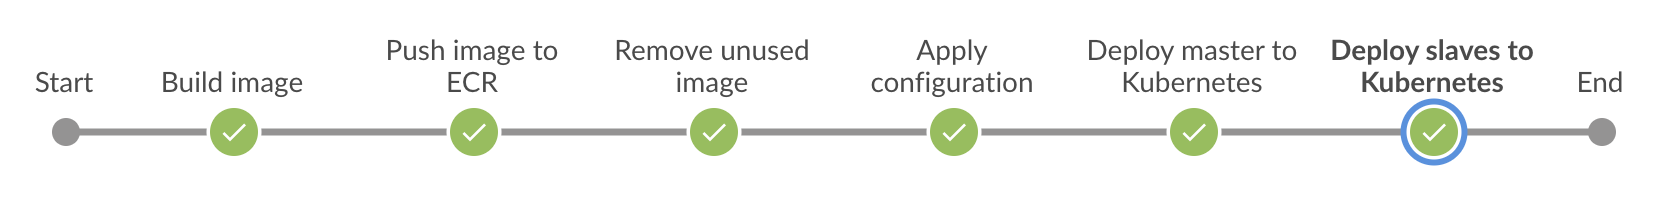
\includegraphics[width=150mm, keepaspectratio]{img/dbjenkins.png}
\caption{Az adatbázistelepítés Jenkinsben végrehajtott lépései}
\end{figure}
\vskip 0.1in
\begin{enumerate}
    \item \textbf{Konténerkép összeállítása} - Erre a lépésre azért van szükség mert egy \lstinline{init.sql} fájlt rá kell másolni a konténerre, így viszont már új kép keletkezik (\textit{megjegyzés: a kezdeti inicializálást Kubernetes ConfigMap segítségével is meg lehetne oldani. Számomra a Docker képfájl a lokális tesztelés során volt kényelmes}). Ezzel történik az adatbázis inicializálása az első telepítéskor (frissítés során értelemszerűen nem).
    \item \textbf{Konténerkép feltöltése ECRbe} - Ahhoz hogy a Kubernetes hozzáférjen az előbb épített képhez ahhoz ECRbe kell feltölteni.
    \item \textbf{Nem használt kép eltávolítása} - A Docker-in-Docker konténer megőrzi a képet alapértelmezetten. Ezt ki kell törölni hogy ne teljen meg a lemezterület. (Az ECR tárolja a képeket.)
    \item \textbf{Konfiguráció alkalmazása} - Ez alkalmazza a GitHub repositoryban található \textit{Secret} és \textit{ConfigMap} objektumokon végzett változtatásokat.
    \item \textbf{Mesterpéldány telepítése} - A mesterpéldányon végzett módosításokat lépteti érvénybe. Nem jár adatbáziskieséssel ugyanis az alárendelt példányok átveszik a mester szerepét a kiesés idejére.
    \item \textbf{Alárendelt példányok telepítése} - Miután a főpéldány újra készen áll a kiszolgálásra, az alárendelt példányok frissítése is megtörténik.
\end{enumerate}
Az adatbázison összesen a jelszavakat kell konfigurálni, a többi teljesen működőképes állapotba kerül a Jenkins segítségével. Ezt a \lstinline{secrets.yaml} fájlban lehet megtenni. Szükséges egy replikációs jelszó és egy hozzáférési jelszó is. Előbbi csak az adatbázispéldányok közti kommunikációra használatos, nem kell megjegyezni. Utóbbi az alkalmazások/emberek számára is látható, az adminisztrátori hozzáférést biztosítja a telepítés után.
\section{CI és CD megvalósítása}
A Jenkins készen áll arra hogy alkalmazásokat telepítsen Kubernetesbe, az alkalmazások pedig fel vannak erre készítve. Már csak azt kell megoldani hogy a Jenkins tudja, hogy \textit{honnan}, \textit{mikor} és \textit{hogyan} telepítse azokat.
\subsection{Jenkinsfájlok}
A Jenkinsben úgynevezett \textit{Multibranch pipeline} fog létrejönni amikor majd összekötjük a GitHubbal. Ezt azt jelenti, hogy alapértelmezetten amelyik git ágon egy \textit{Jenkinsfile} nevű fájl található, azt a Jenkins számára értelmezettnek tekinti és megkísérli végrehajtani az ott leírt utasításokat.

Egy Jenkinsfile szakaszokból, a szakaszok pedig lépésekből épülnek fel. Ezek a lépések párhuzamosan is végrehajthatóak (bár ez a feladatom során nem volt hasznosítható). Minden szakasznak definiálható továbbá hogy mikor hajtódjon végre. A lépések során használhatunk Docker parancsokat, futtathatunk Shell szkriptet, vagy egyéb szolgáltatásokat is igénybe vehetünk (mivel a Jenkins erősen bővíthető). Ismételten a backend példáján keresztül fogom szemlélteni a működést:
\begin{lstlisting}
def branch_name = "${BRANCH_NAME}" //a branch nevét környezeti változóból groovy változóba helyezzük későbbi használatra
pipeline {
  environment {
    //meghatározzuk a használni kívánt registryt és repositoryt
    registry = "XXXXXXXXXXX.dkr.ecr.eu-central-1.amazonaws.com/webshop-backend"
    registryCredential = 'ecr:eu-central-1:aws' //ez az Amazon hozzáférés amit korábban a Jenkinsben elmentettünk. Formátum: ecr:régió:credential_ID
    dockerImage = '' //ez majd a keletkezett konténerképet fogja tárolni
    IMAGE_TAG = "$BUILD_NUMBER-$BRANCH_NAME" //a konténer tagje lesz a build sorszáma és a branch neve
    NAMESPACE = "webshop-$BRANCH_NAME" //a névtér amibe a kubernetesen belül telepíteni fogunk
    DOMAIN = "mbraptor.tech" //ez a változó később a yaml fájlba fog kerülni
  }
  agent any
  stages {
    stage('Build image') {
      steps{
        script {
          dockerImage = docker.build registry + ":$IMAGE_TAG" //beépített paranccsal konténerképet készítünk
        }
      }
    }
    stage('Push image to ECR') {
      when {
        expression { return branch_name ==~ /(prod|beta)/ } //ha a kitüntetett branch valamelyikén vagyunk csak akkor hajtjuk végre ez a szakaszt
      }
      steps{
        script {
          docker.withRegistry("https://" + registry, registryCredential) {
            dockerImage.push() //adott belépési adatokkal feltöltjük ECRbe a képet
          }
        }
      }
    }
    stage('Remove unused image') {
      when {
        expression { return branch_name ==~ /(prod|beta)/ }
      }
      steps{
        sh(script: "docker rmi $registry:$IMAGE_TAG", returnStdout: true) // töröljük a képet a lokális dockerből
      }
    }
    stage('Deploy to Kubernetes') {
      when {
        expression { return branch_name ==~ /(prod|beta)/ }
      }
      steps{
        sh(script: "envsubst < backend-${BRANCH_NAME}.yaml | kubectl -n $NAMESPACE apply -f - && sleep 10", returnStdout: true) //a változókat a linuxos envsubst program segítségével átírjuk az értékükre (pl.: \$IMAGE\_TAG), majd alkalmazzuk a Kubernetesben a változtatásokat
      }
    }
  }
}
\end{lstlisting}
Ha minden lépés sikerrel lezajlott akkor zöld színű lesz a Jenkins, ellenkező esetben piros, és hibaüzenetet kapunk.
\subsection{GitHub konfigurálása}
Ahhoz hogy a Jenkins példányunk a GitHubon tárolt forráskódhoz hozzáférjen ahhoz be kell konfigurálni egy-két dolgot. Az első lépés a hozzáférés engedélyezése.
Szükségünk lesz egy úgynevezett \textit{GitHub Personal Access Token}re mely gyakorlatilag egy egyszerű szövegfüzér. Ezt a GitHub oldalán a \textbf{Profile} gombra kattintva a \textbf{Settings} alatt a \textbf{Developer settings}nél találjuk. Itt kattintsunk a \textbf{Generate new token} gombra. Az alábbi jogosultságokat adjuk meg:
\begin{itemize}
    \item admin:repo\_hook
    \item read:user
    \item repo
    \item user:email
\end{itemize}
Ezzel kapunk egy hosszabb szöveget mely a token a Jenkins számára. Ezt két helyen kell felhasználni a Jenkinsen belül:
\begin{itemize}
    \item A \textbf{Manage Jenkins, Configure System} útvonalon keressük meg a \textbf{GitHub} részt. Adjunk hozzá egy \textbf{GitHub szerver}t tetszőleges névvel. Az \textbf{API URL} \url{https://api.github.com} a \textbf{Credentials}nál pedig adjunk hozzá egy új \textbf{Secret Text} típusú titkot és másoljuk be a tokent. Válasszuk ki a legördülő menüben az előbb létrehozott titok azonosítóját, illetve jelöljük be a \textbf{Manage Hooks} jelölőnégyzetet.
    \item Nyissuk meg a \textbf{Blue Ocean} nézetet mely a Jenkins új felülete, és válasszuk a \textbf{New Pipeline} lehetőséget. Itt menjünk végig a lépéseken, másoljuk be a tokent és válasszunk egy tetszőleges repositoryt.
\end{itemize}
Ezzel a kapcsolat létrejött a GitHub és a Jenkins között és a Manage Hooks bejelölése miatt a WebHook is megjelenik a GitHub repository megfelelő részén.

A webhookok segítségével a Jenkins valós időben értesül a feliratkozott eseményekről. Erről a GitHub HTTP \textit{POST} kérés formájában értesíti a megadott végpontot.
\begin{figure}[ht]
\centering
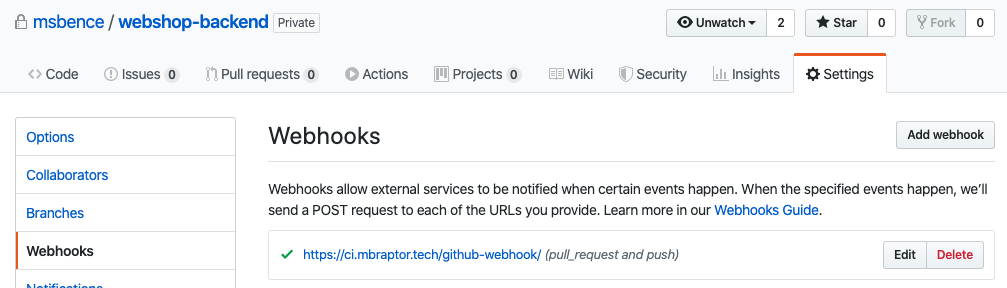
\includegraphics[width=150mm, keepaspectratio]{img/webhook.png}
\caption{A GitHub oldalon megjelenik az új webhook}
\end{figure}
\vskip 0.1in
A másik két alkalmazáskomponens felvétele a Blue Ocean felületen hasonlóan egyszerű.

Még két fontos dolgot kell beállítani, bár ez opcionális, és tervezés kérdése. Én a gyakorlatban alkalmazhatónak gondolom a lentieket, és szeretném megmutatni a lehetőségeket. Célszerű konfigurálni a Jenkins feladatnál, hogy kizárólag a kitüntetett ágakat és a Pull Requesteket vegye figyelembe. Természetesen ahogyan az Jenkinsfileban is látszik, a telepítési/frissítési feladatok ettől a beállítástól függetlenül, kizárólag csak a két főágon hajtódnak végre. Válasszünk ki egy Jenkins feladatot a \textbf{hagyományos} felületen, ekkor bal oldalt megjelenik a \textbf{Configure} lehetőség. Itt válasszük a \textbf{Branch Sources} fület, és adjunk hozzá egy RegEx\footnote{Regular Expressions - reguláris kifejezések, gyakorlatilag egy szűrőkifejezés mely szövegre illetszthető} szűrőt a következő értékkel: \lstinline{(prod|beta|PR.+)} (tehát a \textit{prod} vagy \textit{beta} vagy a \textit{PR-} kezdetű branchek (a pull requestek a Jenkinsben PR-ként jelennek meg)).
\begin{figure}[ht]
\centering
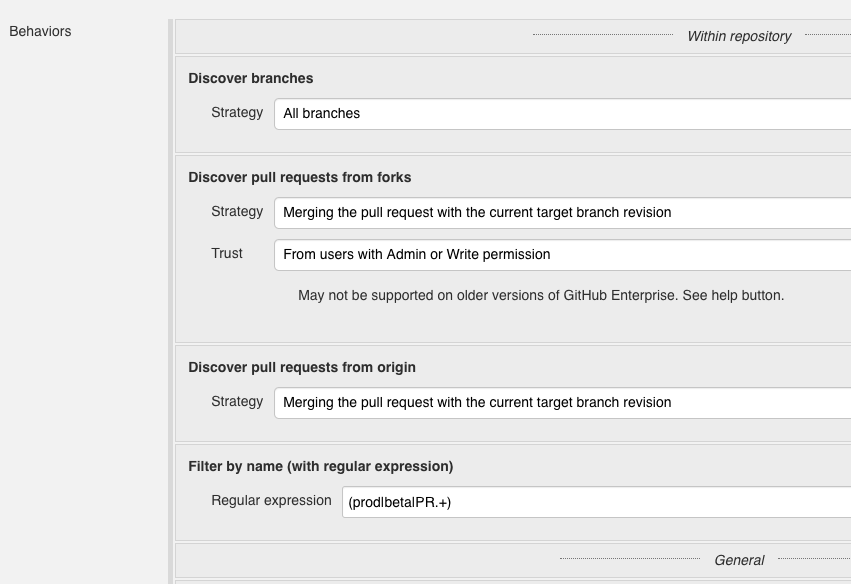
\includegraphics[width=150mm, keepaspectratio]{img/jenkinsbranch.png}
\caption{Ágak szűrése Jenkins és RegEx segítségével}
\end{figure}
\newpage
A másik hasznos lehetőség a korábban említett \textit{Branch Protection} alkalmazása. Ezt GitHubon kell konfigurálni egy adott repositoryn belül. A megfelelő beállításokkal "védetté" tehetjük az adott ágat, például csak akkor olvaszhatunk bele módosításokat, ha a Jenkins azt leellenőrizte. Konfigurálható még továbbá, hogy egy fejlesztőnek kötelező átnéznie azt. Ahhoz, hogy a Jenkins ellenőrzést kötelezővé tudjuk tenni, ahhoz a GitHubnak regisztrálnia kell annak létezését, amihez viszont egy Pull Requestnek léteznie kell. Csináljunk egyet, később törölhetjük, nem kell elfogadni sem. Most már látni fogja a GitHub a Jenkins ellenőrzés létezését, állítsuk is be. A repository \textbf{Settings} fülén válasszuk bal oldalt a \textbf{Branches} részt, és a \textbf{Branch Protection Rules}nál adjunk hozzá egy új szabályt az \textbf{Add rule} gombra kattintva. A \textbf{Branch name pattern}nél adjuk meg a védeni kívánt branch nevét (sajnos jelenleg áganként külön szabályt kell felvinni), és jelöljük be a \textbf{Require status checks to pass before merging} négyzetet, azon belül pedig a \textbf{Require branches to be up to date before merging} négyzetet. A Jenkins ellenőrzést a \textbf{continuous-integration/jenkins/pr-merge} bejelölésével kapcsolhatjuk be. Érdemes még engedélyezni a force pusht (\textbf{Allow force pushes}), ugyanis a Git használata során ez bizonyos esetekben (rebase) teljesen indokolt lehet.
\begin{figure}[ht]
\centering
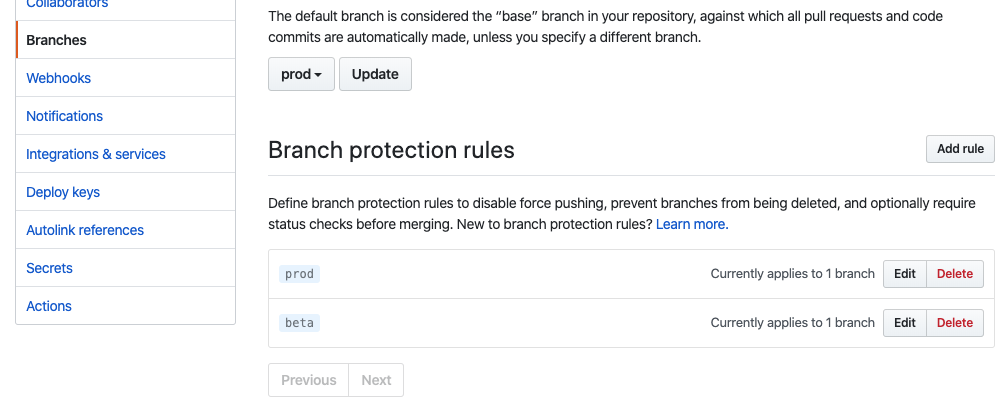
\includegraphics[width=150mm, keepaspectratio]{img/gitbranch.png}
\caption{Az fontos ágak védve vannak}
\end{figure}

Ezekkel a beállításokkal gyakorlatilag a feladat \textit{Continuous Integration} része is elkészült, most már biztosak lehetünk benne hogy az általunk választott ágakon kizárólag Jenkins által ellenőrzött kód található, az azzal való munka során egészen biztosan egy működő állapotból indulunk ki.
\newpage
\subsection{Alkalmazás telepítése és frissítése}
Miután a fentieket az összes alkalmazáskomponenesre elvégeztük gyakorlatilag végeztük is. Ha mindent jól csináltunk, akkor amikor a Jenkinsbe regisztráltuk a GitHub repositorykat akkor az végrehajtotta az összes lépést és ez a telepítést is magában foglalja. Innentől kezdve ha egy Pull Request (\textit{ami szintén ellenőrizve lesz, csupán a frissítéssel kapcsolatos lépések maradnak ki}) elfogadásra kerül, tehát a főágba lesz olvasztva akkor a Jenkins végrehajtja azon az ágon is a teljes folyamatot, azonban itt már minden lépést, tehát az alkalmazáskomponens frissítve lesz, mégpedig leállás nélkül, tekintettel arra, hogy minden egységnél definiáltunk \textit{Readiness Probe}ot, a Kubernetes pedig alapértelmezésben egyesével cseréli a futó példányokat. Ezzel elkészült egy teljes CI/CD alkalmazás.
\begin{figure}[ht]
\centering
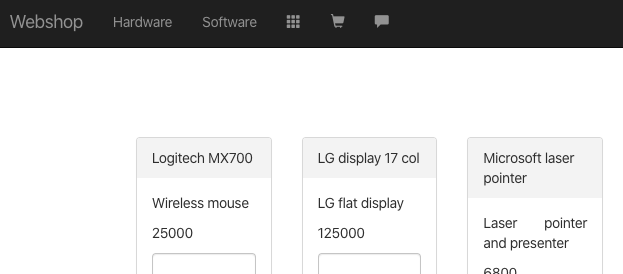
\includegraphics[width=120mm, keepaspectratio]{img/appprod.png}
\vskip 0.2in
%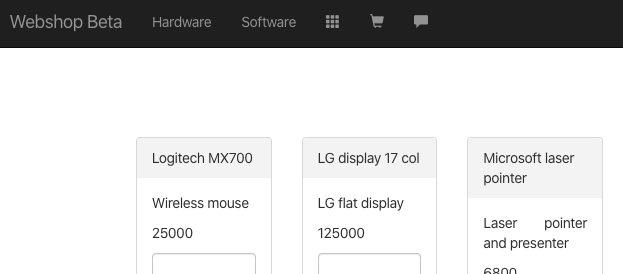
\includegraphics[width=120mm, keepaspectratio]{img/appbeta.png}
%\vskip 0.2in
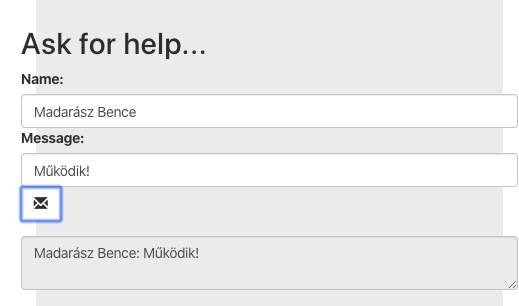
\includegraphics[width=120mm, keepaspectratio]{img/appchat.png}
\caption{A működő webáruház és chatfelülete}
\end{figure}